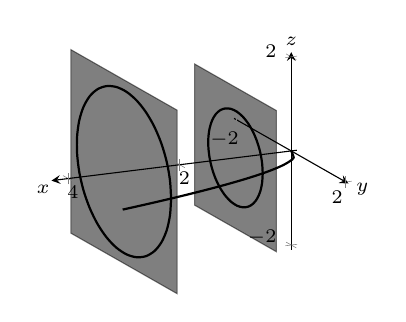
\begin{tikzpicture}[>=stealth]
\begin{axis}%
[width=175pt,tick label style={font=\scriptsize},axis on top,
			axis lines=center,
			view={155}{20},
			name=myplot,
			%xtick=\empty,
			%ytick=\empty,
			%ztick=\empty,
			ymin=-2.1,ymax=2.1,
			xmin=-.1,xmax=4.3,
			zmin=-2.1, zmax=2.1,
			every axis x label/.style={at={(axis cs:\pgfkeysvalueof{/pgfplots/xmax},0,0)},xshift=-3pt,yshift=-3pt},
				xlabel={\scriptsize $x$},
			every axis y label/.style={at={(axis cs:0,\pgfkeysvalueof{/pgfplots/ymax},0)},xshift=5pt,yshift=-2pt},
				ylabel={\scriptsize $y$},
				every axis z label/.style={at={(axis cs:0,0,\pgfkeysvalueof{/pgfplots/zmax})},xshift=0pt,yshift=4pt},
				zlabel={\scriptsize $z$}
			]

%\addplot3[domain=0:180,smooth,y domain=0:360,surf,%fill=white,
%colormap={mp2}{\colormapplaneone},faceted color=black!40,samples=30,samples y=25,very thin,z buffer=sort] ({cos(x)*1.5*cos(y)},{sin(x)*cos(y)},{sin(y)});





\filldraw[draw={\coloronefill},fill={\coloronefill},opacity=.5] (axis cs: 1,1.5,1.5) -- (axis cs:1,1.5,-1.5) -- (axis cs:1,-1.5,-1.5) -- (axis cs:1,-1.5,1.5) -- cycle;

\addplot3[domain=0:360,,thick,smooth,samples y=0,{\colortwo},%surf,%fill=white,
samples=30,] ({1},{cos(x)},{sin(x)});

\filldraw[draw={\coloronefill},fill={\coloronefill},opacity=.5] (axis cs: 3,1.95,1.95) -- (axis cs:3,1.95,-1.95) -- (axis cs:3,-1.95,-1.95) -- (axis cs:3,-1.95,1.95) -- cycle;

\addplot3[domain=0:360,,thick,smooth,samples y=0,{\colortwo},%surf,%fill=white,
samples=30,] ({3},{1.73*cos(x)},{1.73*sin(x)});

\addplot3[domain=0:4,,thick,smooth,samples y=0,{\colorone},%surf,%fill=white,
samples=30,] ({x},{sqrt(x)},{0});

\end{axis}


\end{tikzpicture}












